% Homework report template for courses lectured by Blaz Zupan.
% For more on LaTeX please consult its documentation pages, or
% read tutorials like http://tobi.oetiker.ch/lshort/lshort.pdf.
%
% Use pdflatex to produce a PDF of a report.

\documentclass[a4paper,11pt]{article}
\usepackage{a4wide}
\usepackage{fullpage}
\usepackage[utf8x]{inputenc}
\usepackage[toc,page]{appendix}
\usepackage[pdftex]{graphicx} % for figures
\usepackage{setspace}
\usepackage{color}
\definecolor{light-gray}{gray}{0.95}
\usepackage{listings} % for inclusion of Python code
\usepackage{hyperref}
\renewcommand{\baselinestretch}{1.2}

\lstset{ % style for Python code, improve if needed
language=Python,
basicstyle=\footnotesize,
basicstyle=\ttfamily\footnotesize\setstretch{1},
backgroundcolor=\color{light-gray},
}

\title{Homework \#5: Network of Diseases}
\author{Anže Pečar (63060257)}
\date{\today}

\begin{document}

\maketitle

\section{Introduction}

In homework \#5 we build a network of diseases from the OMIM database. We use a network clustering algorithm by Raghavan et al and the python networkx library.

\section{Data}

We get the list of Diseases and their genes from the OMIM morbidmap file. Because some records are very similar we use some simple heuristic to group them. 

We constructed the graph following this simple principle: if two diseases share a gene their corresponding graph nodes should be connected. As seen in the Figure \ref{scale} the graph is not scale free. The diameter of the largest connected component is 12.

\section{Methods}

To cluster similar diseases we used  the network clustering algorithm with label propagation by Raghavean et al. The algorithm is actually quite simple. You choose a random node in the graph, and find it's neighbours. Once you have all the neighbours you rename your original node with the most common label from the neighbours. If there is more than one label tied to be the most common you choose a random one.

\section{Results}
In both Figure \ref{components} and Figure \ref{scale} we could not use $pylab.scale("log")$ as the graph would be drawn in a weird way. Our solution is not perfect as the y axis values can be misleading.

As seen in Figure \ref{dis}, the networkx library didn't do the best job with the spring layout (even though we tried using as much as 3000 iterations). Nevertheless it can be seen how at least some of the similar disease nodes tend to stick together.

Figures \ref{cancer} \ref{deaf} and \ref{diab} show all the extracted clusters "Breast cancer", "Deafness", and "Diabetes mellitus". I am not an expert, but it seems to me that the clustering algorithm did a decent job. We can see that the algorithm grouped some other cancers together with Breast cancer which seems to show that clustering has indeed worked.

\begin{figure}[h!]
\begin{center}
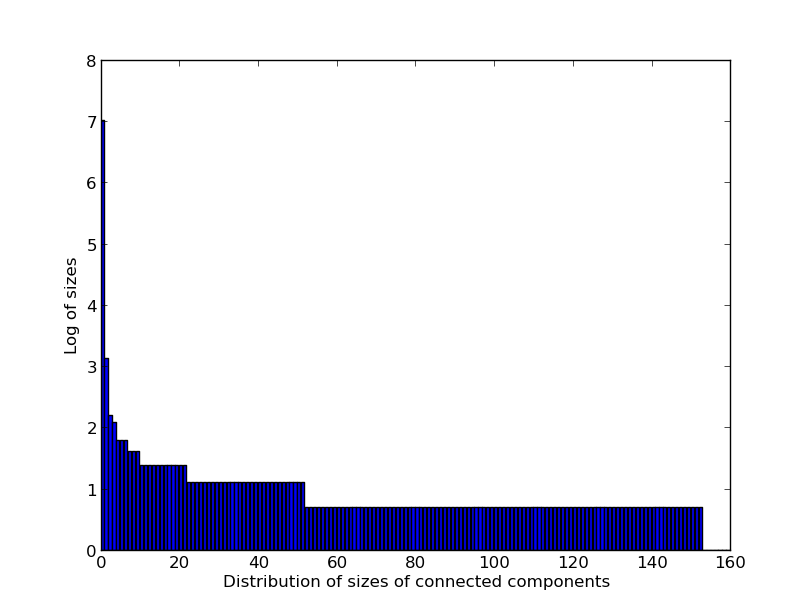
\includegraphics[scale=0.50]{components.png}
\caption{Distribution of sizes of connected components}
\label{components}
\end{center}
\end{figure}


\begin{figure}[h!]
\begin{center}
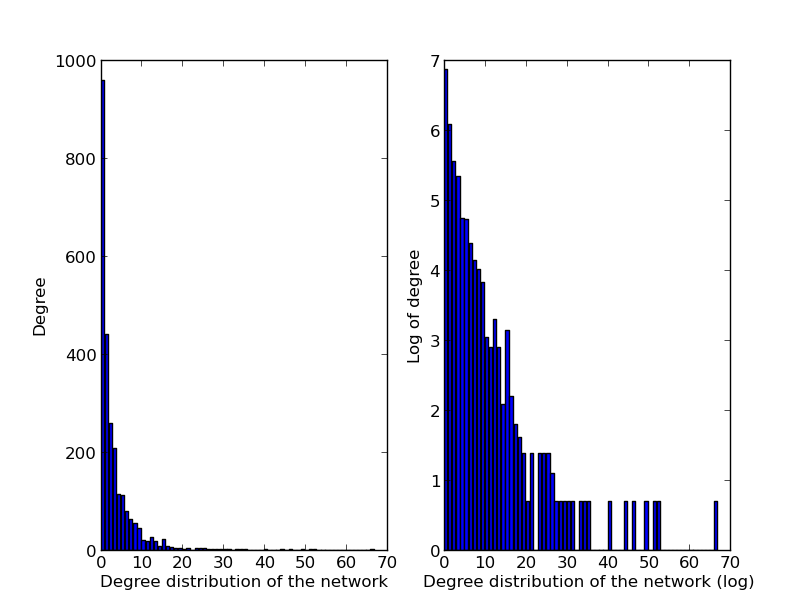
\includegraphics[scale=0.50]{scale.png}
\caption{Degree distribution of the network with and without log}
\label{scale}
\end{center}
\end{figure}

\begin{figure}[h!]
\begin{center}
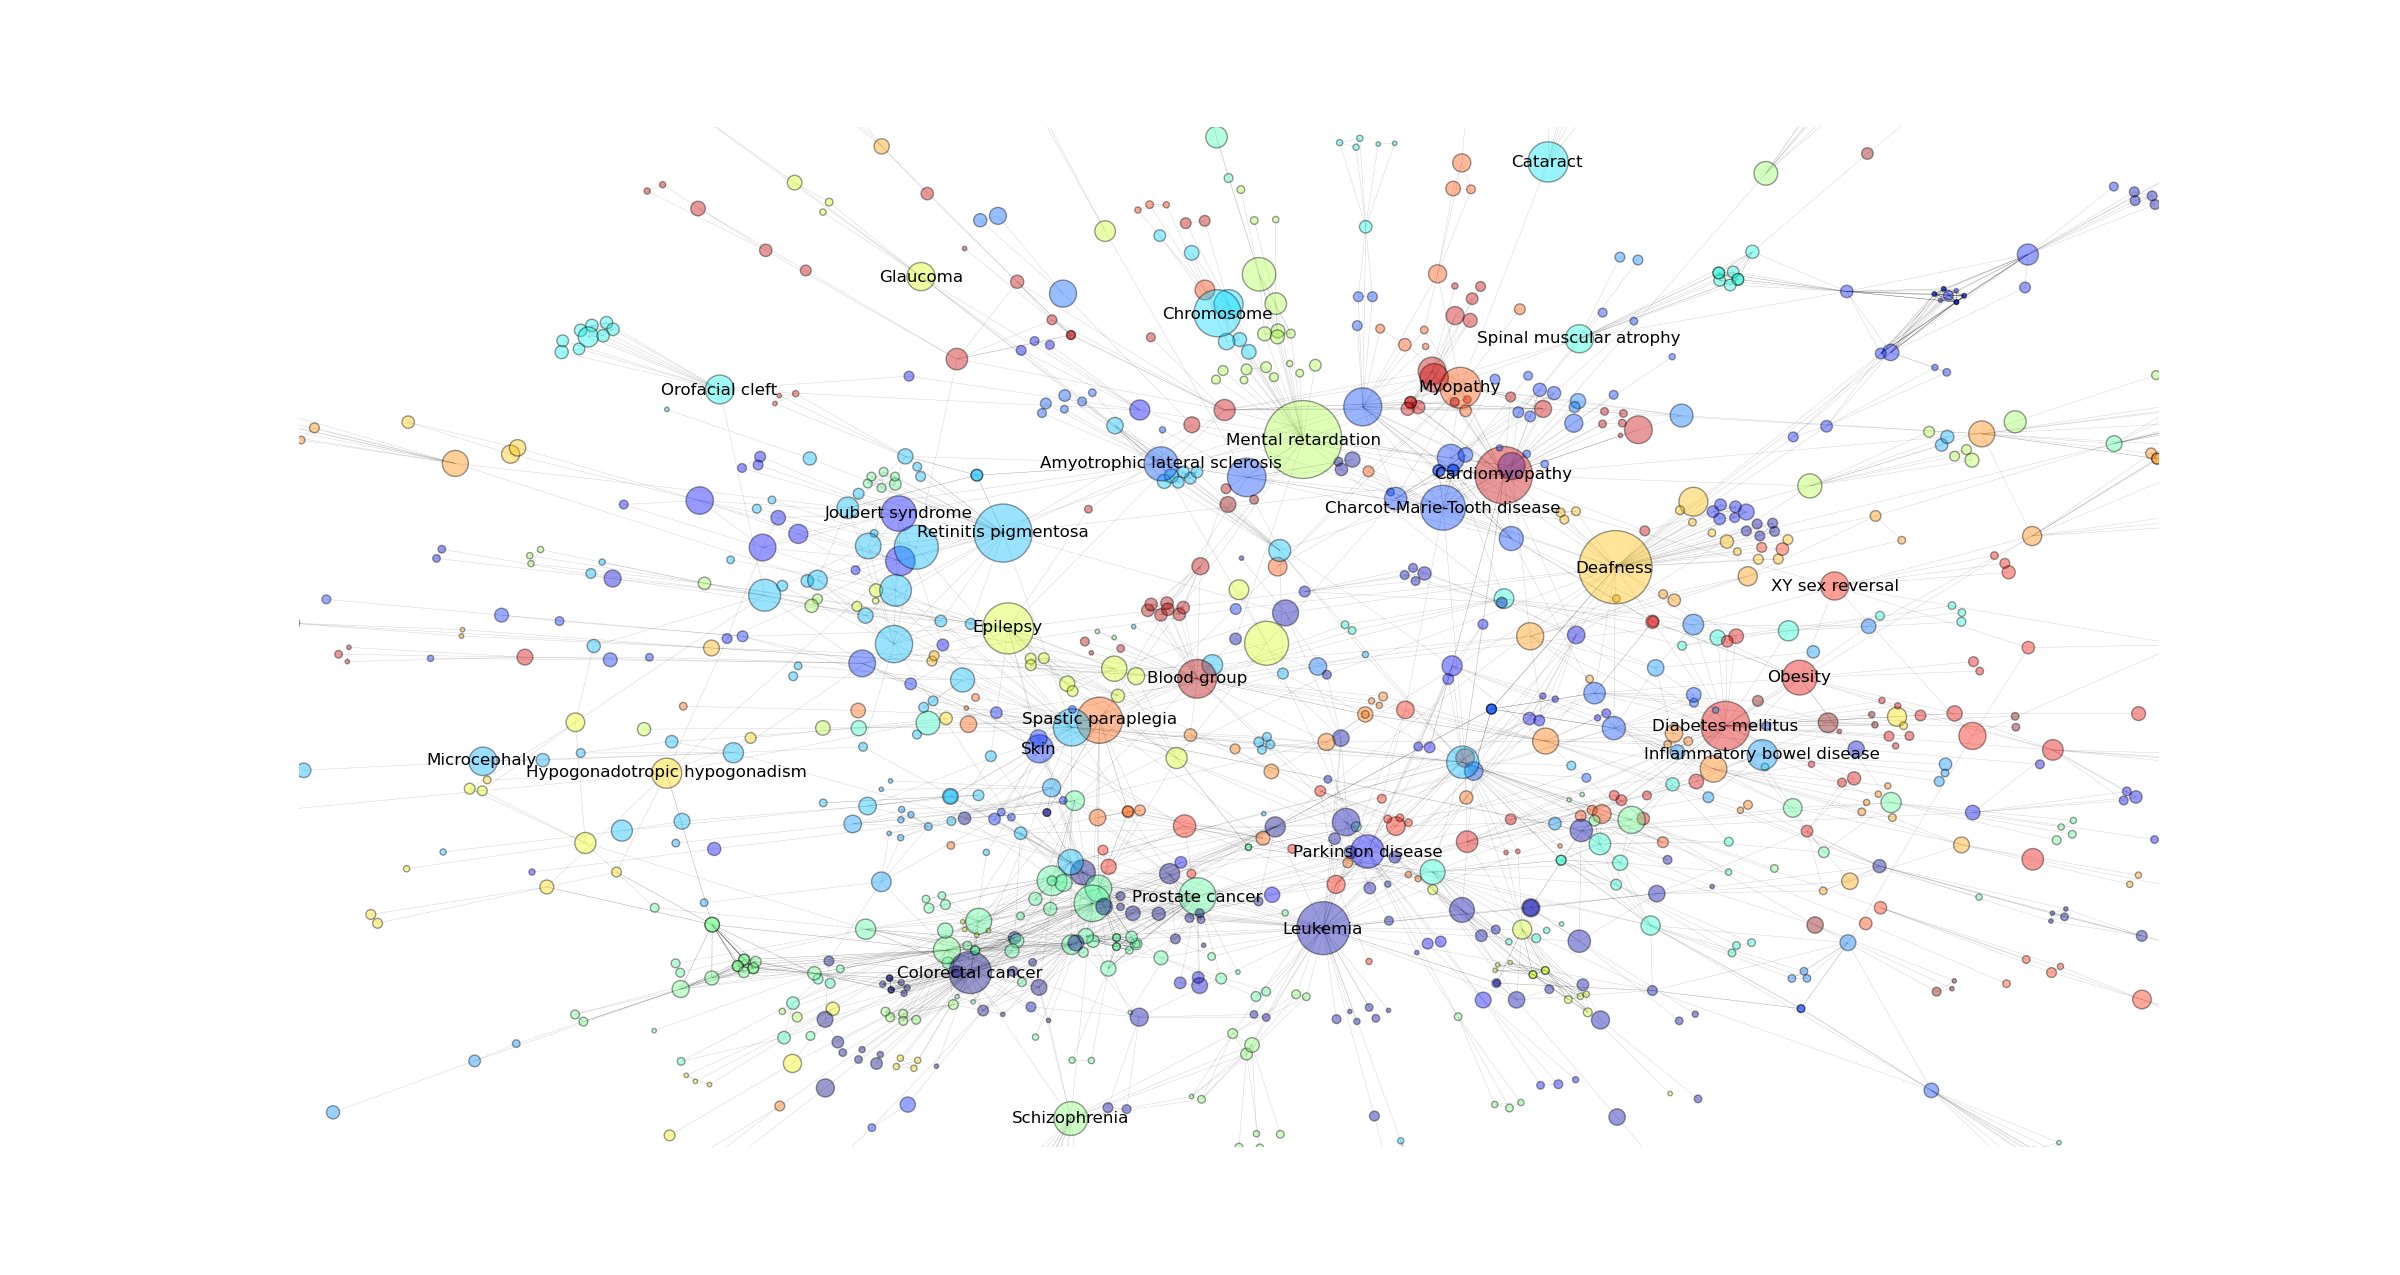
\includegraphics[scale=0.20]{disease.png}
\caption{Largest connected component of your network}
\label{dis}
\end{center}
\end{figure}

\begin{figure}[h!]
\begin{center}
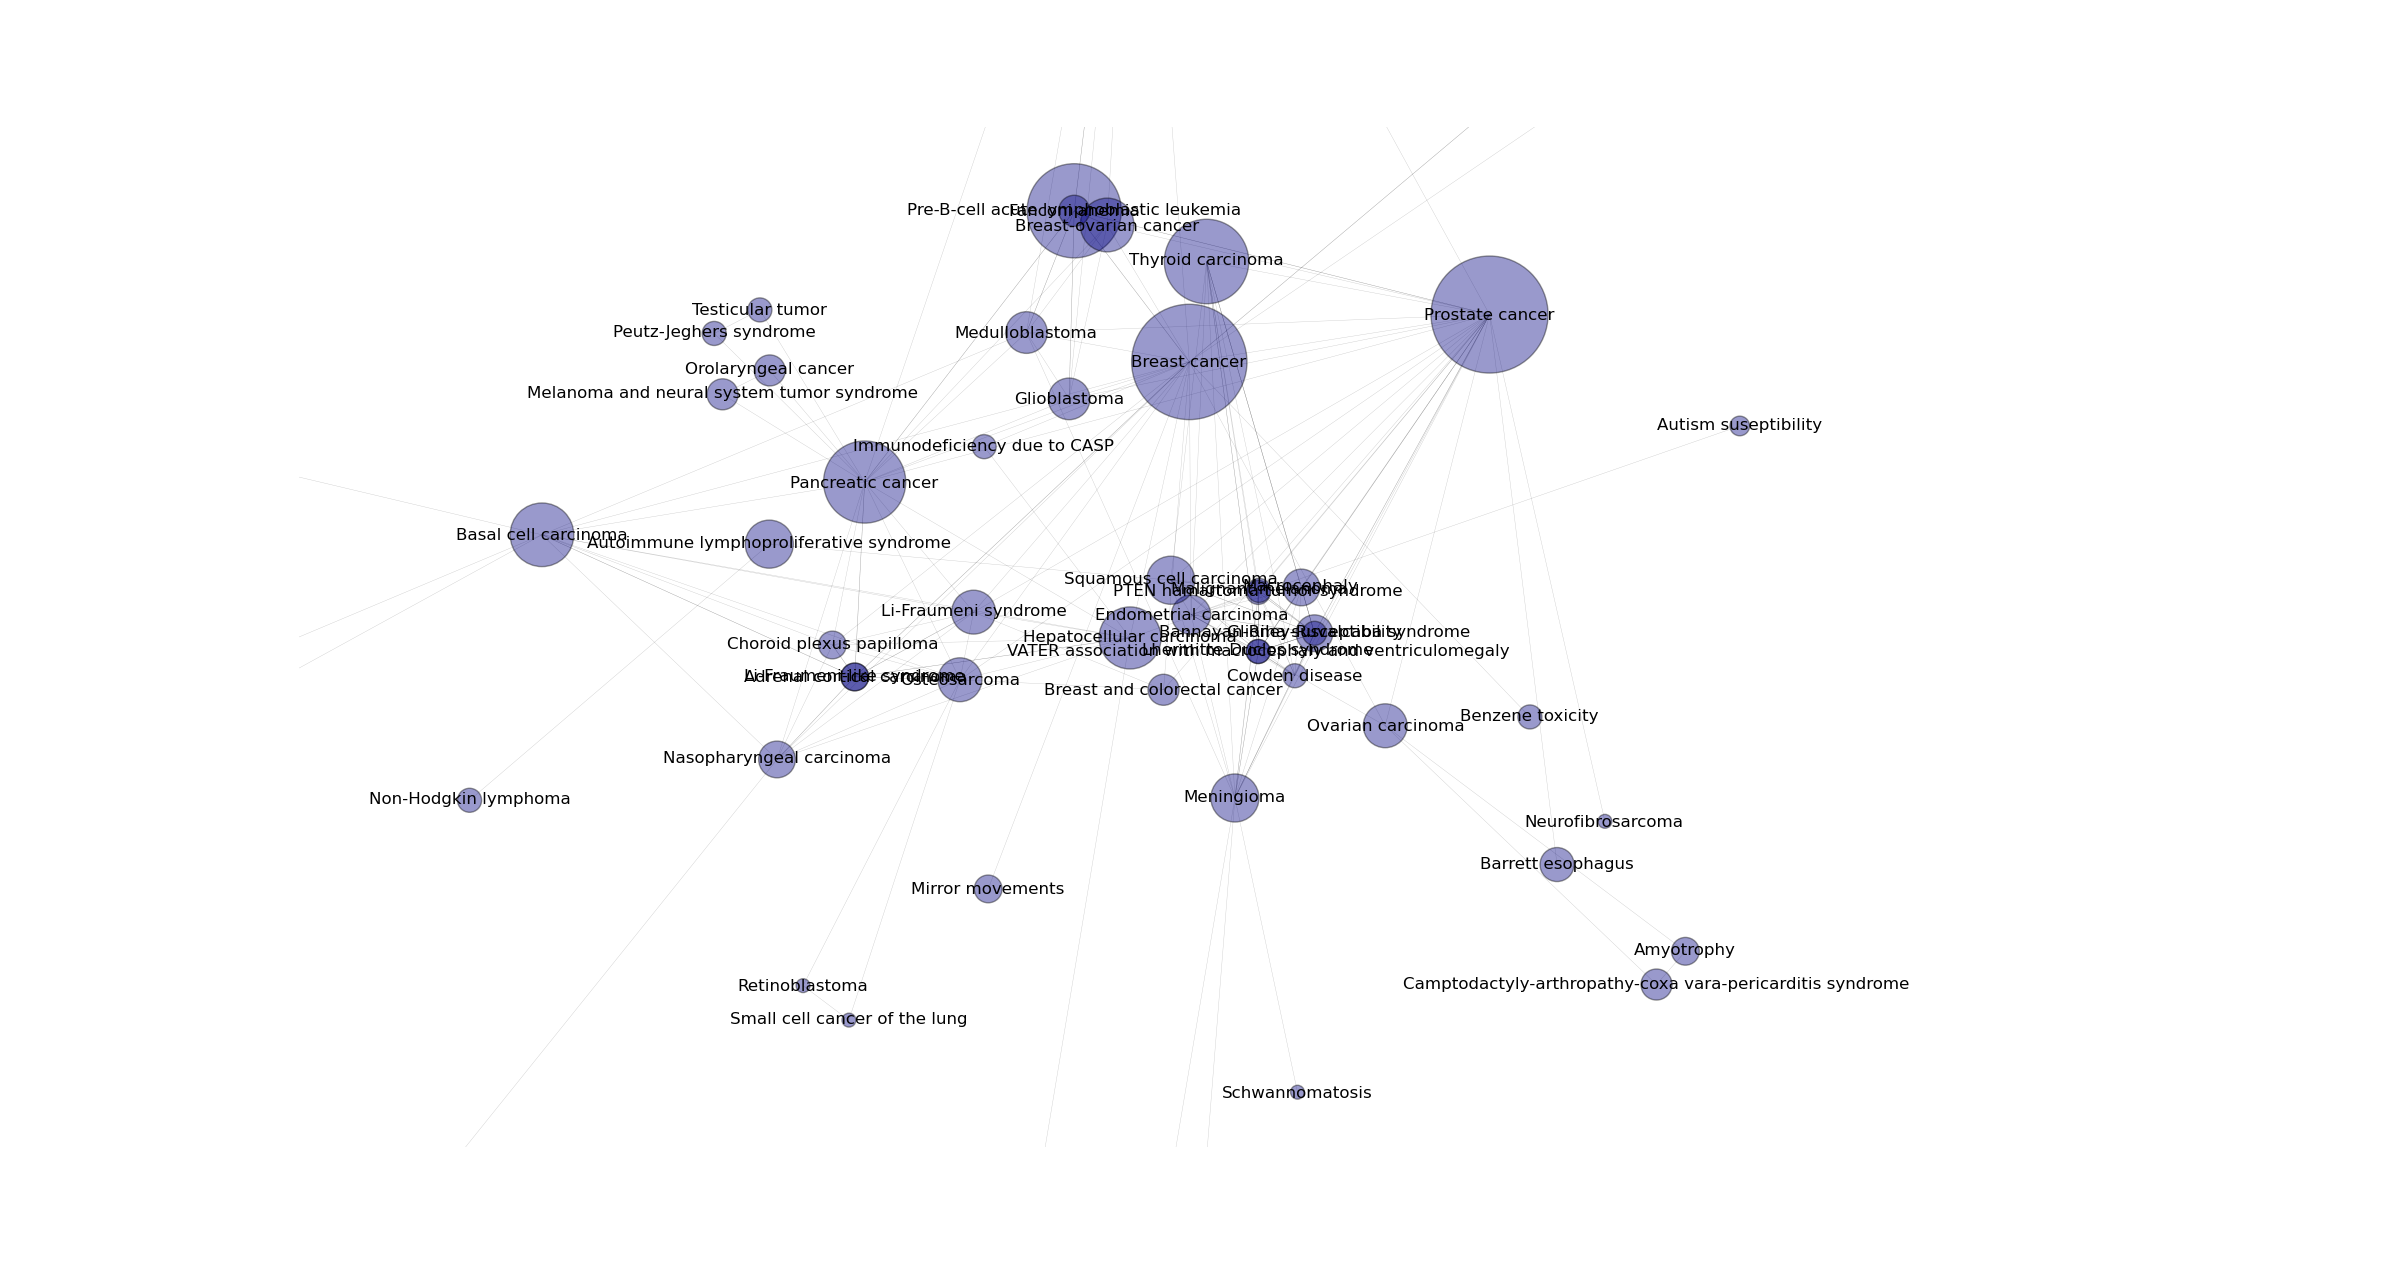
\includegraphics[scale=0.30]{cancer.png}
\caption{Breast cancer cluster}
\label{cancer}
\end{center}
\end{figure}

\begin{figure}[h!]
\begin{center}
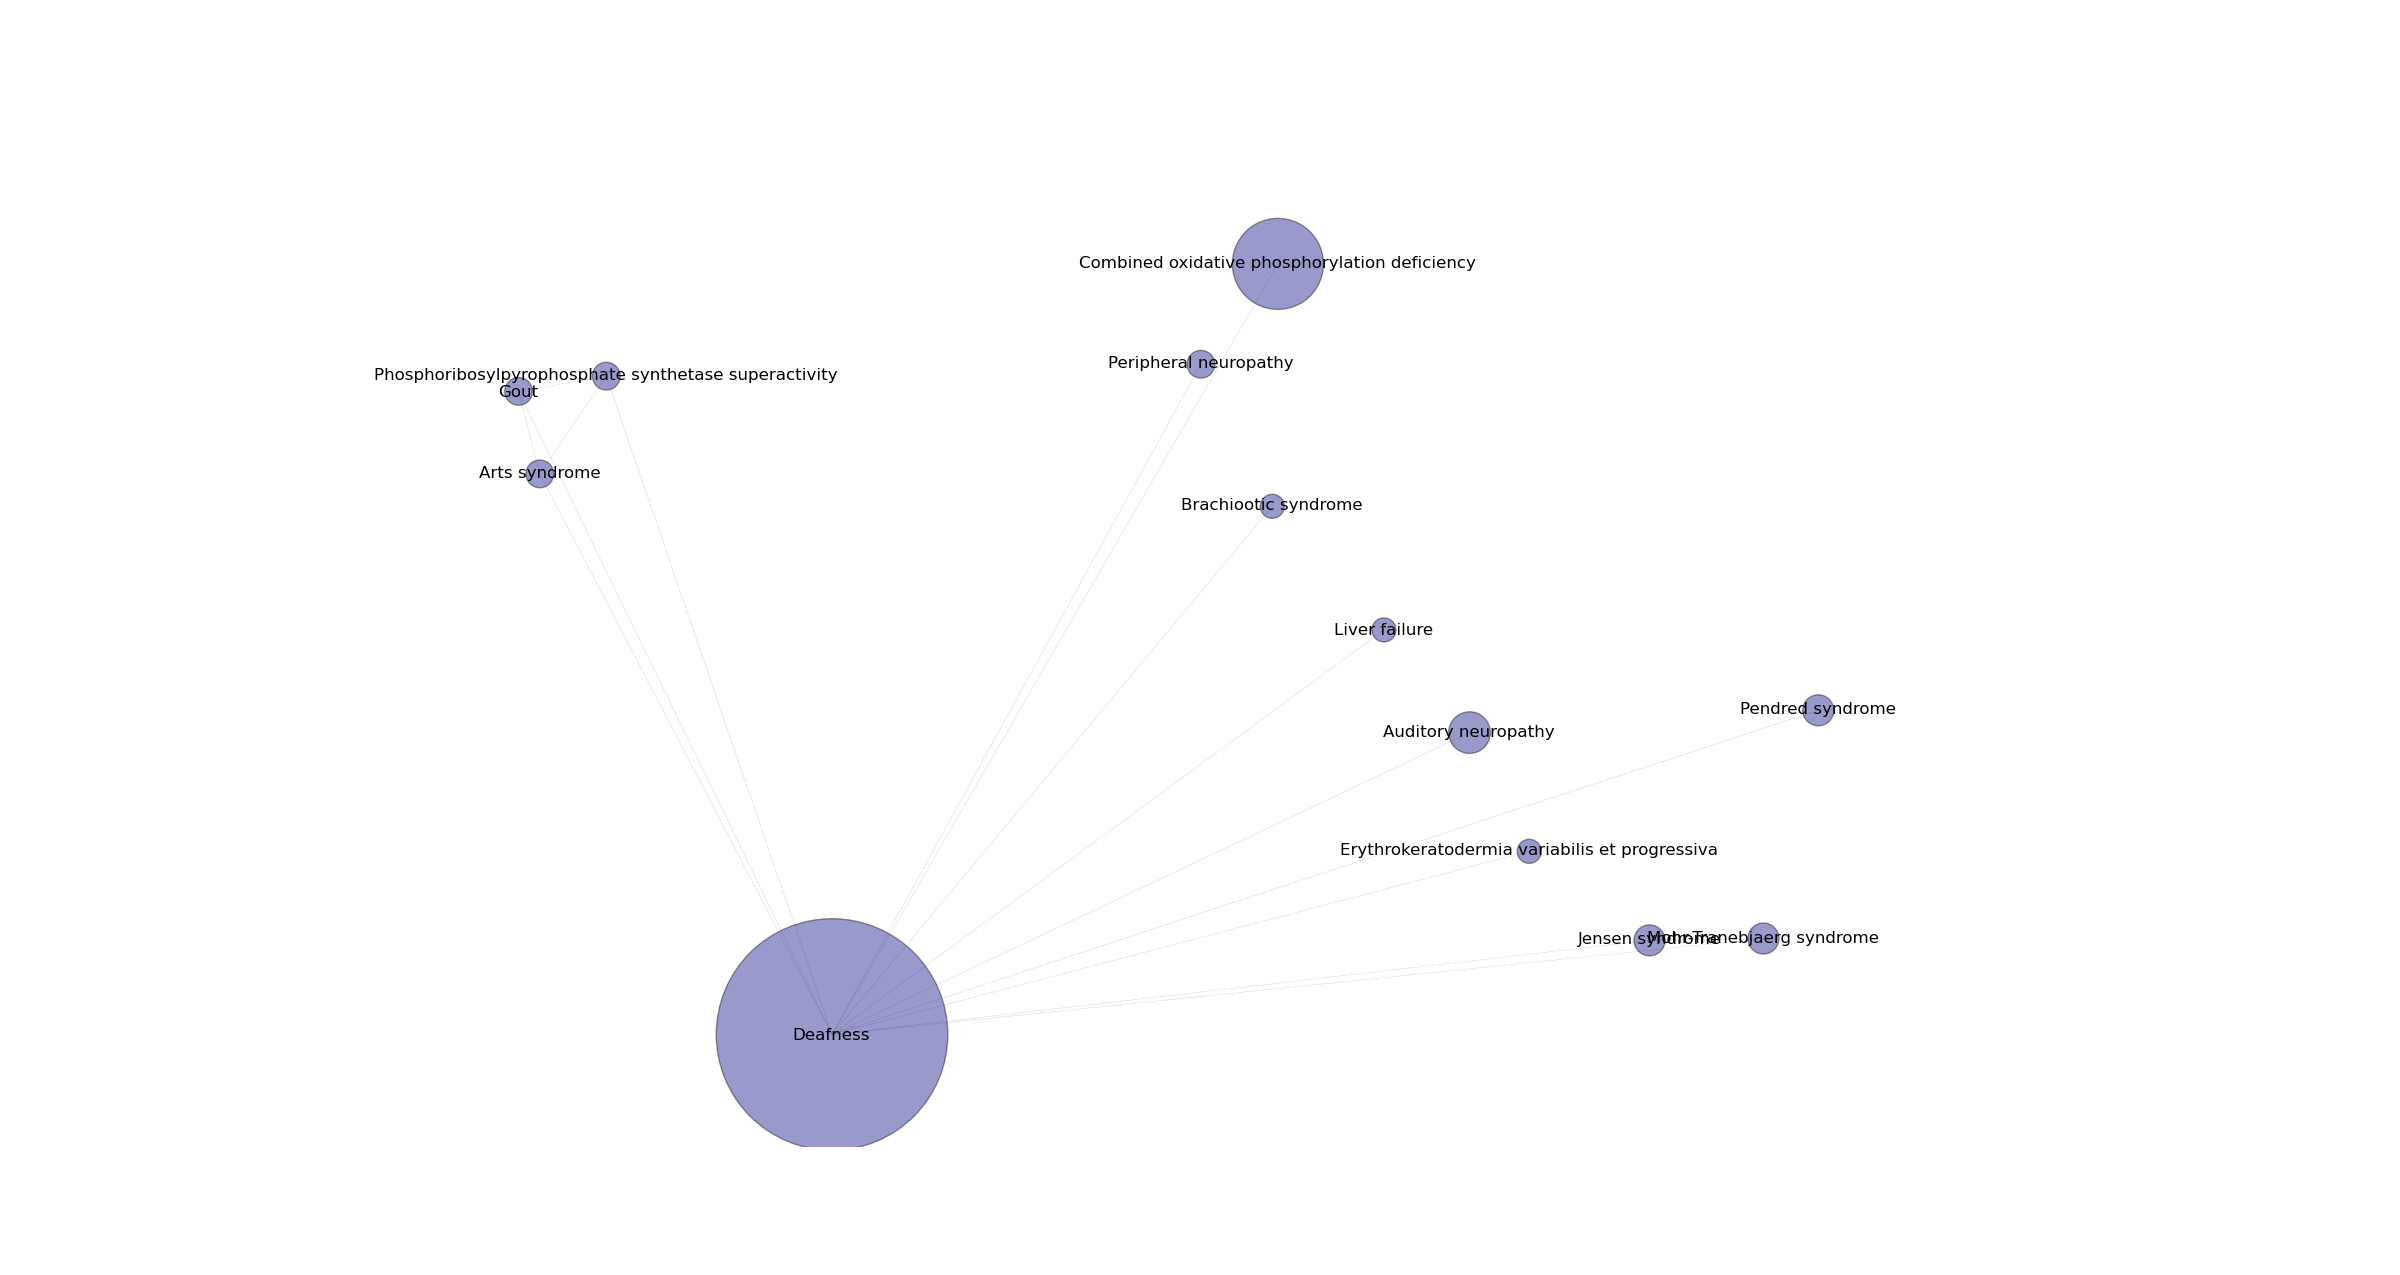
\includegraphics[scale=0.30]{deafness.png}
\caption{Deafness cluster}
\label{deaf}
\end{center}
\end{figure}

\begin{figure}[h!]
\begin{center}
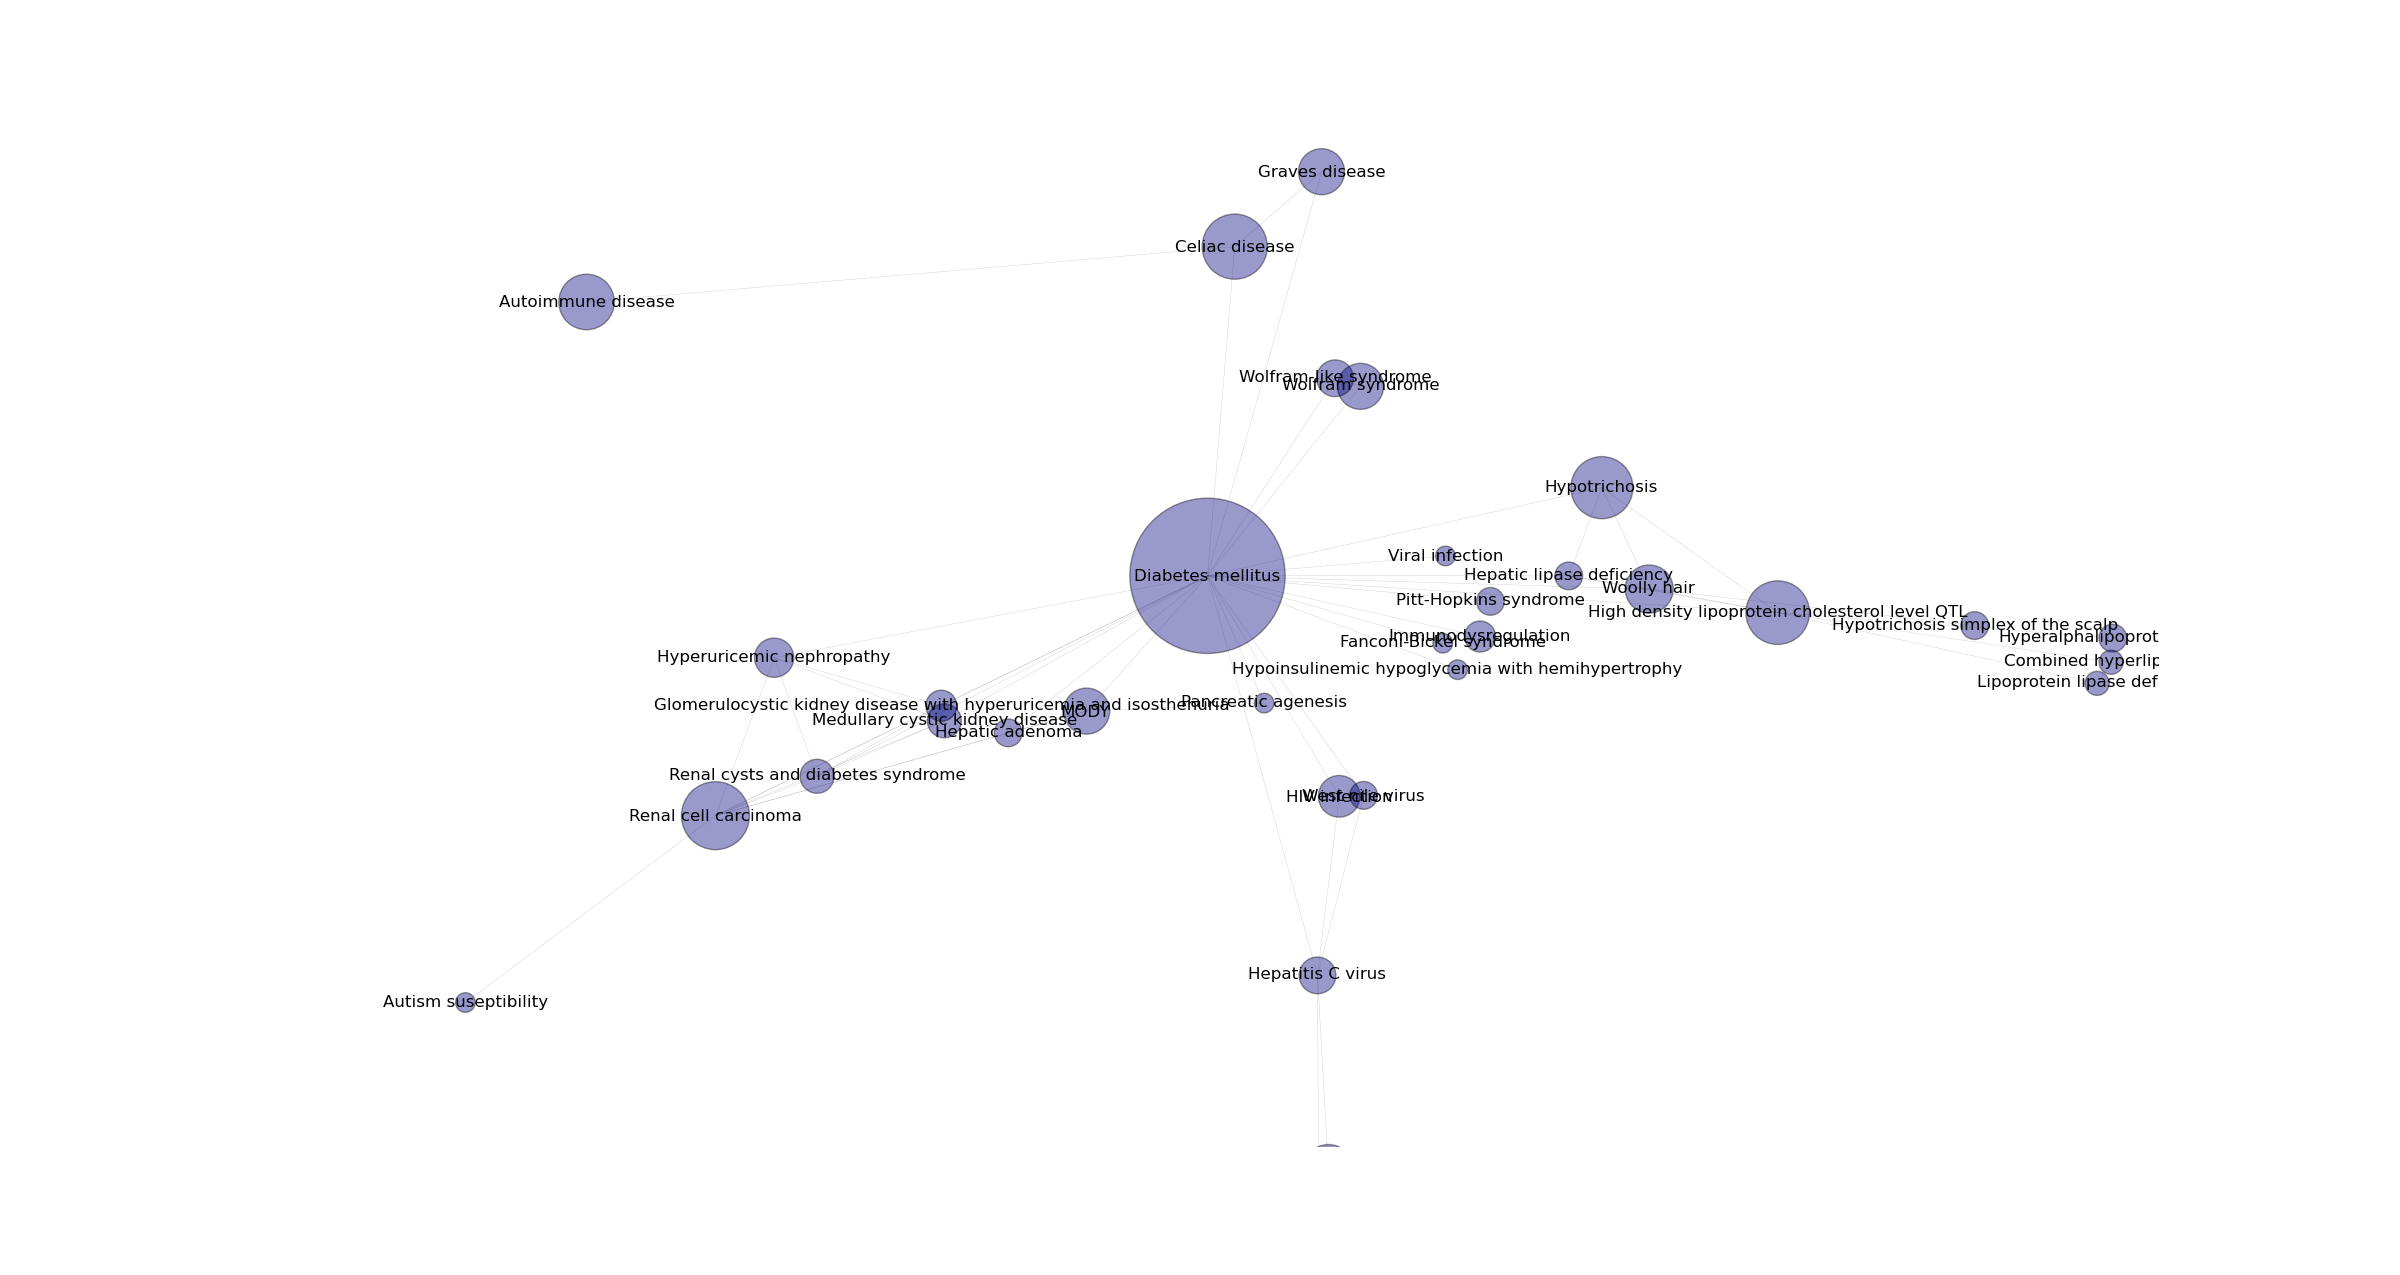
\includegraphics[scale=0.30]{diab.png}
\caption{Diabetes mellitus cluster}
\label{diab}
\end{center}
\end{figure}

\section*{Honor Code}

% The following paragraph of your report should be included as is - do % not change it.

My answers to homework are my own work. I did not make solutions or code available to anyone else. I did not engage in any other activities that will dishonestly improve my results or dishonestly improve/hurt the results of others.


\end{document}